\documentclass[tikz,border=10pt]{standalone}
\usepackage{tikz}
\usetikzlibrary{shapes.geometric, arrows.meta, positioning, fit, backgrounds, calc, decorations.pathreplacing}
\usepackage{amsmath}
\usepackage{xcolor}

% 定义颜色
\definecolor{normalgreen}{RGB}{76, 175, 80}
\definecolor{maliciousred}{RGB}{244, 67, 54}
\definecolor{uncertainorange}{RGB}{255, 152, 0}
\definecolor{serverblue}{RGB}{33, 150, 243}
\definecolor{committeepurple}{RGB}{156, 39, 176}
\definecolor{tlbocyan}{RGB}{0, 188, 212}
\definecolor{evidencegray}{RGB}{158, 158, 158}
\definecolor{lightbg}{RGB}{245, 245, 245}

\begin{document}
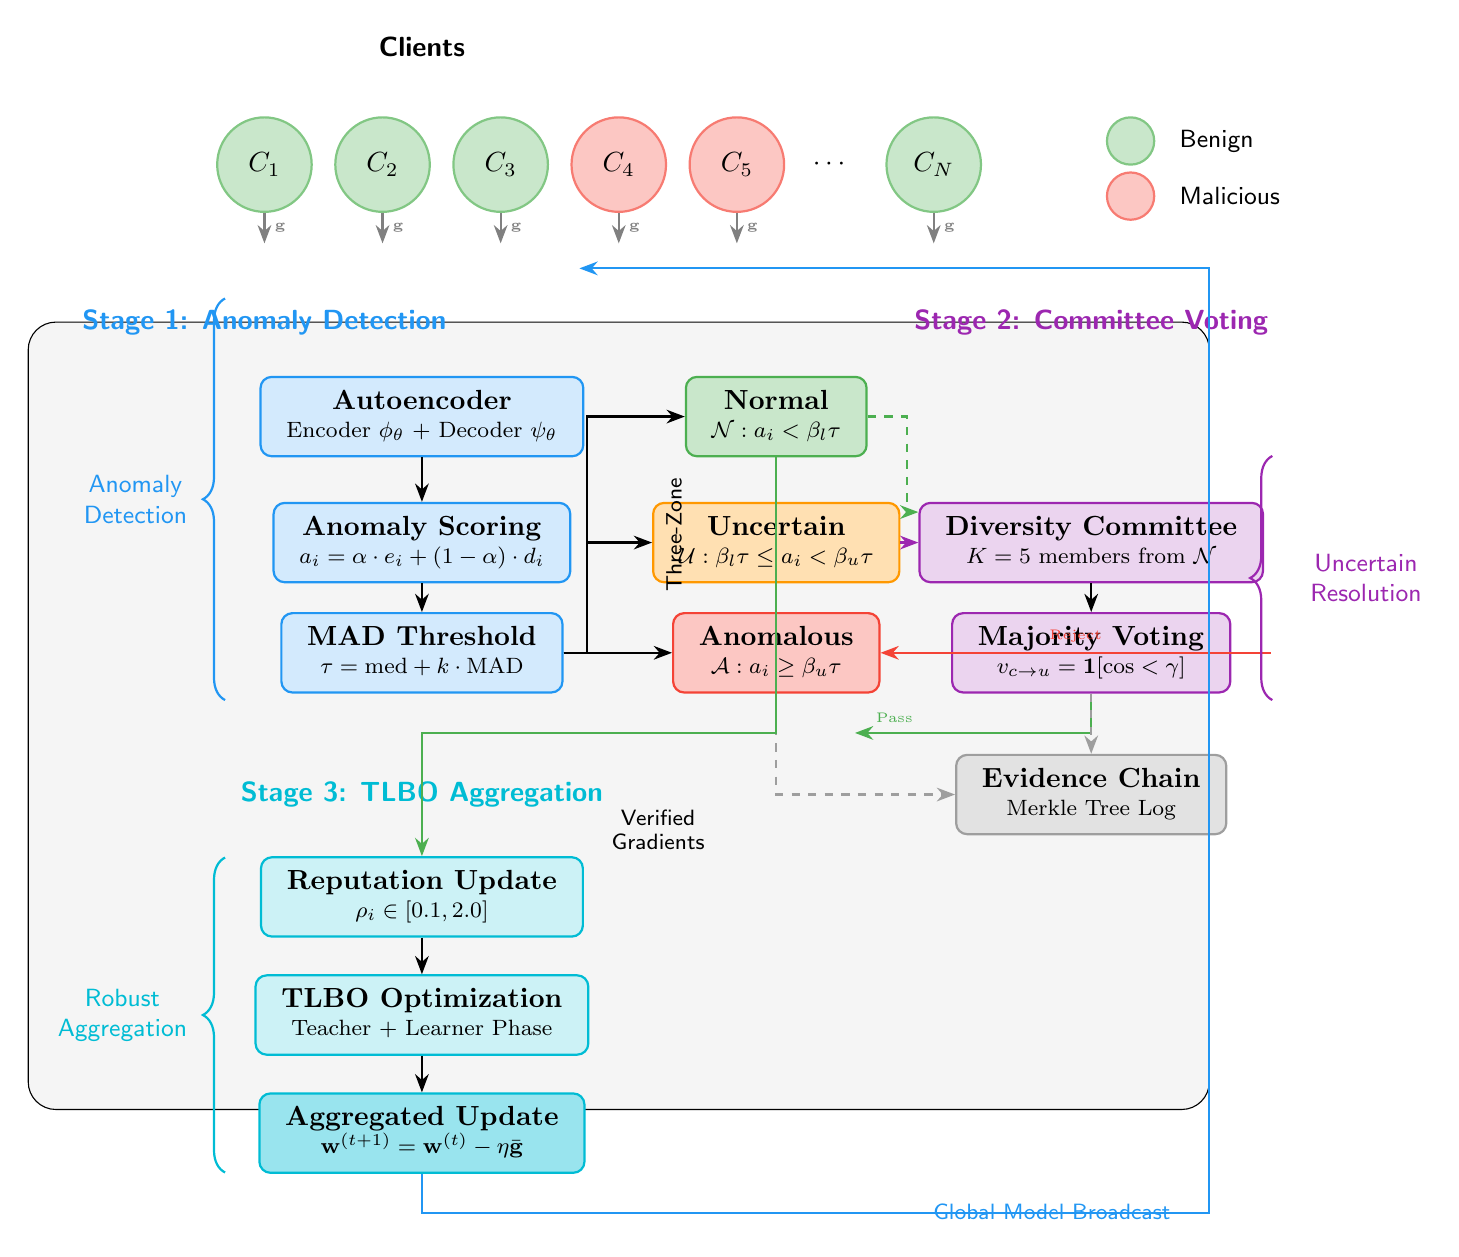
\begin{tikzpicture}[
    node distance=0.8cm and 1.2cm,
    >={Stealth[length=2mm]},
    client/.style={draw, circle, minimum size=1.2cm, thick},
    normalclient/.style={client, fill=normalgreen!30, draw=normalgreen!70},
    maliciousclient/.style={client, fill=maliciousred!30, draw=maliciousred!70},
    serverbox/.style={draw, rounded corners, fill=serverblue!10, draw=serverblue, thick, minimum width=3cm, minimum height=1.5cm},
    processbox/.style={draw, rounded corners, fill=white, thick, minimum width=2.5cm, minimum height=1cm},
    zonebox/.style={draw, rounded corners, thick, minimum width=1.8cm, minimum height=0.8cm},
    arrowstyle/.style={->, thick, >=Stealth},
    dashedarrow/.style={->, thick, dashed, >=Stealth},
    label/.style={font=\small\sffamily},
]

% ==================== 客户端层 ====================
\node[font=\bfseries\sffamily] at (-4, 5.5) {Clients};

% 正常客户端
\node[normalclient] (c1) at (-6, 4) {$C_1$};
\node[normalclient] (c2) at (-4.5, 4) {$C_2$};
\node[normalclient] (c3) at (-3, 4) {$C_3$};

% 恶意客户端
\node[maliciousclient] (c4) at (-1.5, 4) {$C_4$};
\node[maliciousclient] (c5) at (0, 4) {$C_5$};

% 更多客户端省略
\node[font=\sffamily] at (1.2, 4) {$\cdots$};
\node[normalclient] (cn) at (2.5, 4) {$C_N$};

% 客户端图例
\node[normalclient, minimum size=0.6cm] at (5, 4.3) {};
\node[font=\small\sffamily, right] at (5.5, 4.3) {Benign};
\node[maliciousclient, minimum size=0.6cm] at (5, 3.6) {};
\node[font=\small\sffamily, right] at (5.5, 3.6) {Malicious};

% 梯度箭头
\foreach \c in {c1, c2, c3, c4, c5, cn} {
    \draw[arrowstyle, gray] (\c) -- ++(0, -1) node[midway, right, font=\tiny] {$\mathbf{g}$};
}

% ==================== 服务器边界 ====================
\begin{scope}[on background layer]
    \node[draw, rounded corners=10pt, fill=lightbg, minimum width=15cm, minimum height=10cm, 
          label={[font=\bfseries\sffamily]above:Federated Server}] (serverarea) at (-1.5, -3) {};
\end{scope}

% ==================== Stage 1: Autoencoder检测 ====================
\node[font=\bfseries\sffamily\color{serverblue}] at (-6, 2) {Stage 1: Anomaly Detection};

% Autoencoder模块
\node[processbox, fill=serverblue!20, draw=serverblue, minimum width=4cm] (ae) at (-4, 0.8) {
    \begin{tabular}{c}
    \textbf{Autoencoder}\\[-2pt]
    \footnotesize Encoder $\phi_\theta$ + Decoder $\psi_\theta$
    \end{tabular}
};

% 异常评分
\node[processbox, fill=serverblue!20, draw=serverblue, minimum width=3.5cm] (score) at (-4, -0.8) {
    \begin{tabular}{c}
    \textbf{Anomaly Scoring}\\[-2pt]
    \footnotesize $a_i = \alpha \cdot e_i + (1-\alpha) \cdot d_i$
    \end{tabular}
};

% 自适应阈值
\node[processbox, fill=serverblue!20, draw=serverblue, minimum width=3.5cm] (threshold) at (-4, -2.2) {
    \begin{tabular}{c}
    \textbf{MAD Threshold}\\[-2pt]
    \footnotesize $\tau = \text{med} + k \cdot \text{MAD}$
    \end{tabular}
};

% 箭头连接
\draw[arrowstyle] (ae) -- (score);
\draw[arrowstyle] (score) -- (threshold);

% ==================== 三区分类 ====================
% Normal区
\node[zonebox, fill=normalgreen!30, draw=normalgreen] (normal) at (0.5, 0.8) {
    \begin{tabular}{c}
    \textbf{Normal}\\[-2pt]
    \footnotesize $\mathcal{N}: a_i < \beta_l\tau$
    \end{tabular}
};

% Uncertain区
\node[zonebox, fill=uncertainorange!30, draw=uncertainorange] (uncertain) at (0.5, -0.8) {
    \begin{tabular}{c}
    \textbf{Uncertain}\\[-2pt]
    \footnotesize $\mathcal{U}: \beta_l\tau \le a_i < \beta_u\tau$
    \end{tabular}
};

% Anomalous区
\node[zonebox, fill=maliciousred!30, draw=maliciousred] (anomalous) at (0.5, -2.2) {
    \begin{tabular}{c}
    \textbf{Anomalous}\\[-2pt]
    \footnotesize $\mathcal{A}: a_i \ge \beta_u\tau$
    \end{tabular}
};

% 三区分类箭头
\draw[arrowstyle] (threshold.east) -- ++(.3,0) |- (normal.west);
\draw[arrowstyle] (threshold.east) -- ++(.3,0) |- (uncertain.west);
\draw[arrowstyle] (threshold.east) -- ++(.3,0) |- (anomalous.west);

% 三区分类标签
\node[font=\footnotesize\sffamily, rotate=90] at (-0.8, -0.7) {Three-Zone};

% ==================== Stage 2: 委员会投票 ====================
\node[font=\bfseries\sffamily\color{committeepurple}] at (4.5, 2) {Stage 2: Committee Voting};

% 委员会模块
\node[processbox, fill=committeepurple!20, draw=committeepurple, minimum width=3.5cm] (committee) at (4.5, -0.8) {
    \begin{tabular}{c}
    \textbf{Diversity Committee}\\[-2pt]
    \footnotesize $K=5$ members from $\mathcal{N}$
    \end{tabular}
};

% 投票决策
\node[processbox, fill=committeepurple!20, draw=committeepurple, minimum width=3.5cm] (vote) at (4.5, -2.2) {
    \begin{tabular}{c}
    \textbf{Majority Voting}\\[-2pt]
    \footnotesize $v_{c \to u} = \mathbf{1}[\cos < \gamma]$
    \end{tabular}
};

% 委员会箭头
\draw[arrowstyle, committeepurple] (uncertain.east) -- (committee.west);
\draw[arrowstyle, normalgreen, dashed] (normal.east) -- ++(0.5,0) |- (committee.170);
\draw[arrowstyle] (committee) -- (vote);

% 投票结果箭头
\draw[arrowstyle, normalgreen] (vote.south) -- ++(0, -0.5) -| ++(-2.5, 0) node[midway, above, font=\tiny] {Pass} -- ++(-0.5, 0);
\draw[arrowstyle, maliciousred] (vote.east) -- ++(0.5, 0) |- (anomalous.east) node[near end, above, font=\tiny] {Reject};

% ==================== 证据链记录 ====================
\node[processbox, fill=evidencegray!30, draw=evidencegray, minimum width=2.5cm] (evidence) at (4.5, -4) {
    \begin{tabular}{c}
    \textbf{Evidence Chain}\\[-2pt]
    \footnotesize Merkle Tree Log
    \end{tabular}
};

% 证据箭头
\draw[dashedarrow, evidencegray] (anomalous.south) |- (evidence.west);
\draw[dashedarrow, evidencegray] (vote.south) -- ++(0, -0.3) -| (evidence.north);

% ==================== Stage 3: TLBO聚合 ====================
\node[font=\bfseries\sffamily\color{tlbocyan}] at (-4, -4) {Stage 3: TLBO Aggregation};

% 信誉权重
\node[processbox, fill=tlbocyan!20, draw=tlbocyan, minimum width=3cm] (reputation) at (-4, -5.3) {
    \begin{tabular}{c}
    \textbf{Reputation Update}\\[-2pt]
    \footnotesize $\rho_i \in [0.1, 2.0]$
    \end{tabular}
};

% TLBO优化
\node[processbox, fill=tlbocyan!20, draw=tlbocyan, minimum width=3cm] (tlbo) at (-4, -6.8) {
    \begin{tabular}{c}
    \textbf{TLBO Optimization}\\[-2pt]
    \footnotesize Teacher + Learner Phase
    \end{tabular}
};

% 聚合输出
\node[processbox, fill=tlbocyan!40, draw=tlbocyan, thick, minimum width=3cm] (aggregate) at (-4, -8.3) {
    \begin{tabular}{c}
    \textbf{Aggregated Update}\\[-2pt]
    \footnotesize $\mathbf{w}^{(t+1)} = \mathbf{w}^{(t)} - \eta \bar{\mathbf{g}}$
    \end{tabular}
};

% 验证梯度流入
\node[font=\footnotesize\sffamily] at (-1, -4.3) {Verified};
\node[font=\footnotesize\sffamily] at (-1, -4.6) {Gradients};
\draw[arrowstyle, normalgreen, thick] (normal.south) -- ++(0, -3.5) -| (reputation.north);

% TLBO内部箭头
\draw[arrowstyle] (reputation) -- (tlbo);
\draw[arrowstyle] (tlbo) -- (aggregate);

% ==================== 全局模型分发 ====================
\draw[arrowstyle, thick, serverblue] (aggregate.south) -- ++(0, -0.5) -- ++(10, 0) -- ++(0, 12) -- ++(-8, 0);
\node[font=\footnotesize\sffamily\color{serverblue}] at (4, -9.3) {Global Model Broadcast};

% ==================== 装饰性大括号 ====================
\draw[decorate, decoration={brace, amplitude=8pt, mirror}, thick, serverblue] 
    (-6.5, 2.3) -- (-6.5, -2.8) node[midway, left=10pt, font=\small\sffamily, align=center] {Anomaly\\Detection};

\draw[decorate, decoration={brace, amplitude=8pt, mirror}, thick, committeepurple] 
    (6.8, 0.3) -- (6.8, -2.8) node[midway, right=10pt, font=\small\sffamily, align=center] {Uncertain\\Resolution};

\draw[decorate, decoration={brace, amplitude=8pt, mirror}, thick, tlbocyan] 
    (-6.5, -4.8) -- (-6.5, -8.8) node[midway, left=10pt, font=\small\sffamily, align=center] {Robust\\Aggregation};

\end{tikzpicture}
\end{document}
